% hello
\documentclass{article}

\usepackage[utf8]{inputenc}
\usepackage{graphicx}
\usepackage[dvipsnames]{xcolor}
\usepackage{csquotes}
\usepackage{hyperref}
\usepackage{tabularx}
\usepackage{booktabs}
\usepackage{pdfpages}
\usepackage{caption,geometry}
\usepackage[toc,page]{appendix}
\newcommand\myshade{85}
\colorlet{mylinkcolor}{violet}
\colorlet{mycitecolor}{YellowOrange}
\colorlet{myurlcolor}{Aquamarine}

\hypersetup{
  linkcolor  = mylinkcolor!\myshade!black,
  citecolor  = mycitecolor!\myshade!black,
  urlcolor   = myurlcolor!\myshade!black,
  colorlinks = true,
}

\usepackage[acronym]{glossaries}

\usepackage{listings}
\lstset{
    frame=Trbl,
    numbers=left,
    breaklines=true,
    basicstyle=\ttfamily,
    postbreak=\mbox{\textcolor{red}{$\hookrightarrow$}\space}
}

\usepackage[maxnames=3,style=authoryear,natbib=true]{biblatex}
\addbibresource{./references.bib}
% \bibliographystyle{unsrtnat}
% \setcitestyle{authoryear}


\newglossary[bsg]{bus}{bsd}{bsn}{Bussiness glossary}
\newglossary[dmg]{dm}{dmd}{dmn}{Data mining glossary}

\graphicspath{ {../images/} }

\DeclareUnicodeCharacter{2008}{-}% support older LaTeX versions
\DeclareUnicodeCharacter{2003}{ }% support older LaTeX versions

\let\oldautoref\autoref
\renewcommand{\autoref}[1]{(\oldautoref{#1})}
\newcommand{\autorefsub}[2]{(\oldautoref{#1}, #2)}
\newcommand{\gmt}{\acrshort{gmt}}
\newcommand{\firstvis}{first-visit data }
\newcommand{\secondvis}{second-visit data }

\newcommand{\uu}{Utrecht University}
\newcommand{\flup}{\gls{d:flup} }
\newcommand{\simon}{\gls{d:simon} }
\newcommand{\dpaper}{the \flup paper }
\newcommand{\Dpaper}{The \flup paper }
\newcommand{\spaper}{the \simon paper }

\newcommand{\MyTitle}[1]{
    \title{
    {#1}\\
    {\large Utrecht University}\\
    }
    \author{Mike Vink}
    \date{ \today }
    \maketitle
}
\newcommand{\f}[3]{%
\begin{figure}[htpb]
    \includegraphics[width=\textwidth]{#1}
    \caption{#2}
    \label{#3}
\end{figure}
}

\newcommand{\fptable}[5]{%

\newgeometry{scale=1}
\thispagestyle{empty}

\begin{table}
{%
    \centering
    \includegraphics[scale=.7]{#1}
    \captionsetup{width=0.8\linewidth}
    \captionof{table}{\textbf{#3} #4}
    \par
    \label{#5}
}
\end{table}

\restoregeometry
}

\newcommand{\fpfig}[5]{%

\newgeometry{scale=1}
\thispagestyle{empty}

\begin{figure}
{%
    \centering
    \includegraphics[scale=.7]{#1}
    \captionsetup{width=0.8\linewidth}
    \captionof{figure}{\textbf{#3} #4}
    \par
    \label{#5}
}
\end{figure}

\restoregeometry
}



\makeglossaries
\newglossaryentry{bu:rnaVirus}
{
    type=bus,
    name=ribonucleic acid virus(es),
    description={An \acrshort{rna} virus is a virus that has \acrshort{rna} as
    its genetic material. Inside a host cell this material is used to generate
    new virusses. Notable human diseases caused by RNA viruses include the
    common cold and influenza}
}
\newglossaryentry{bu:antigen}
{
    type=bus,
    name=antigen,
    description={In immunology, an antigen is a molecule or molecular
    structure, such as \acrshort{ha} and \acrshort{na}, that can be bound by an
    antigen-specific \gls{bu:antibody} or immune cell receptor.  The presence of
    antigens in the body normally triggers an immune response
    }
}
\newglossaryentry{bu:glycoprotein}
{
    type=bus,
    name=glycoprotein,
    description={Glycoproteins are molecules that comprise protein and
    carbohydrate chains. Many viruses have external glycoproteins that
    help them enter bodily cells, but can also serve to be important
    therapeutic or preventative targets}
}
\newglossaryentry{bu:mutation}
{
    type=bus,
    name=mutation,
    description={Mutation of genetic material occurs thanks to its chemical
    instability. The encoded protein molecules can have single amino acid
    (protein building block) change (minor, but still in many cases significant
    change leading to disease) or wide-range amino acid changes}
}
\newglossaryentry{bu:tiv}
{
    type=bus,
    name=TIV,
    description={
        An inactivated trivalent vaccine is a vaccine consisting of \gls{bu:antigen}ic virus particles from viruses that have been grown in culture and then killed to destroy disease producing capacity.
        In practice vaccines of three main types of influenza were used, hence trivalent
    },
    first={inactivated trivalent vaccines (TIV)}
}
\newglossaryentry{bu:antibody}
{
    type=bus,
    name=antibody,
    description={ Protein used by the immune system to identify and neutralize foreign objects such as pathogenic bacteria     and viruses.
    The antibody recognizes a unique molecule of the pathogen, called an \gls{bu:antigen}}
}
\newglossaryentry{bu:titer}
{
    type=bus,
    name=titer,
    description={
    Titer is a way of expressing concentration.
    Titer testing employs serial dilution to obtain approximate quantitative information from an analytical procedure that inherently only evaluates as positive or negative.
    The titer corresponds to the highest dilution factor that still yields a positive reading
    }
}
\newglossaryentry{bu:tcell}
{
    type=bus,
    name=T-cell,
    description={
        A T cell is a type of \gls{bu:lymphocyte}.
        T cells are one of the important white blood cells of the immune system and play a central role in the adaptive immune response, for example generating antibodies against influenza.
        Groups of specific, T cell subtypes have a variety of important functions in controlling and shaping the adaptive immune response
    }
}
\newglossaryentry{bu:lymphocyte}
{
    type=bus,
    name=lymphocyte,
    description={
        A lymphocyte is a type of white blood cell in the immune system of jawed vertebrates.
        Lymphocytes include \gls{bu:tcell}, and \gls{bu:bcell}.
        These cells work together in the adaptive immune response to generate antibodies against influenza
    }
}
\newglossaryentry{bu:cd8pos}
{
    type=bus,
    name=CD8+ T-cell,
    description={
        A cytotoxic T cell (also known as CD8+ T-cell) is a \gls{bu:tcell} that kills cancer cells, cells that are infected (particularly with viruses), or cells that are damaged in other ways.
        It does so by recognizing specific part of \gls{bu:antigen} and then starting a process that kills the targetted cell
    }
}
\newglossaryentry{bu:cd4pos}
{
    type=bus,
    name=CD4+ T-cell,
    description={
        The T helper cells, also known as CD4+ cells, "help" the activity of other immune cells by releasing \gls{bu:cytokine}s.
        These cells help to polarize the immune response into the appropriate kind depending on the nature of the immunological insult (e.g. virus vs. bacterium)
    }
}
\newglossaryentry{bu:cytokine}
{
    type=bus,
    name=cytokine,
    description={
        Cytokines are a broad and loose category of small proteins important in cell signaling that bind to receptor protein on the outside of (immune) cells to fulfill their signal function
    }
}
\newglossaryentry{bu:pbmc}
{
    type=bus,
    name=PBMC,
    description={
        A peripheral blood mononuclear cell is any peripheral blood cell having a round nucleus.
        These cells consist of \gls{bu:lymphocyte} and \gls{bu:monocyte}s
    },
    first={peripheral blood mononuclear cell (PBMC)}
}
\newglossaryentry{bu:bcell}
{
    type=bus,
    name=B-cell,
    description={
        B-cells produce antibody molecules; however, these antibodies are not secreted.
        Rather, they are presented on the outside of the cell where they serve as a part of B-cell receptors.
        When a B-cell is activated by an antigen, it proliferates and differentiates into an antibody-secreting effector cell, known as a plasmablast or plasma cell
    }
}
\newglossaryentry{bu:monocyte}
{
    type=bus,
    name=monocyte,
    description={
        Monocytes are a type of white blood cell.
        Monocytes and their macrophage and dendritic cell progeny serve three main functions in the immune system.
        These are phagocytosis, antigen presentation, and cytokine production.
        Phagocytosis is the process of uptake of microbes and particles followed by digestion and destruction of this material
    }
}
\newglossaryentry{bu:hai}
{
    type=bus,
    name=HAI,
    description={
        The \acrlong{ha} inhibition assay is used to measure the \gls{bu:titer} of \gls{bu:antibody} against a strain of influenza virus present in the serum.
        Antibody levels are measured before vaccination and 28 days after.
        The antibody levels are used to compute the seroprotection and seroconversion criteria
    },
    first={\acrlong{ha} inhibition assay (HAI)}
}
\newglossaryentry{bu:cmv}
{
    type=bus,
    name=CMV,
    description={
        Cytomegalovirus (CMV) is a common herpesvirus found in humans.
        Like other herpesviruses, it is a life-long infection that remains in a latent state inside the human body, until it is 'reactivated' by appropriate conditions.
        Thought to accelerate aging of the immune system and thereby impairing influenza vaccine response  \citep{van_den_Berg_2019}
    },
    first={cytomegalovirus (CMV)}
}
\newglossaryentry{bu:ebv}
{
    type=bus,
    name=EBV,
    description={
        The Epstein–Barr virus (EBV), is one of the nine known human herpesvirus types in the herpes family, and is one of the most common viruses in humans.
    },
    first={Epstein-Barr virus (EBV)}
}
\newglossaryentry{bu:seropc}
{
    type=bus,
    name=seroconversion and seroprotection,
    description={
        A vaccine is considered succesful if the recipient seroconverted (4-fold or greater rise in antibody against virus after vaccination) and were seroprotected (\acrshort{gmt} \(\ge\) 40) after vaccination.
    }
}
\newglossaryentry{bu:stat}
{
    type=bus,
    name=STAT,
    description={
        A vaccine is considered succesful if the recipient seroconverted (4-fold or greater rise in antibody against virus after vaccination) and were seroprotected (\acrshort{gmt} \(\ge\) 40) after vaccination.
    },
    first={signal transducers and activators of transcription (STAT)}
}



\newglossaryentry{d:model}
{
    type=dm,
    name=model,
    description={model is a model}
}
\newglossaryentry{d:flup}
{
    type=dm,
    name=FluPrint,
    description={Data used in this work}
}
\newglossaryentry{d:simon}
{
    type=dm,
    name=SIMON,
    description={Follow up study used in this work}
}

\newacronym{ha}{HA}{hemagglutinin}
\newacronym{na}{NA}{neuraminidase}
\newacronym{rna}{RNA}{ribonucleic acid}


\begin{document}
\MyTitle{Data Understanding Report}
\tableofcontents
\printglossary[type=bus]
\printglossary[type=dm]
\printglossary[type=\acronymtype]

\section{Initial data collection}

\subsection{Technical description data collection}

\subsubsection{MySQL database set up and data import}

By following the guide on the
\href{https://github.com/LogIN-/fluprint}{FluPrint Github Repository} the MySQL
server was set up. In this work the FluPrint github was first added as a
submodule. This module provides the php scripts to import raw data csv's into
the MySQL database. The operating system and versions of php and MySQL used in
this work were OSX "Big Sur" (on Mac Book air 2017), php 7.3.24 (built-in mac
version), and MySQL 8.0.23 (homebrew).

In the \href{https://github.com/LogIN-/fluprint}{guide} the dependencies to run
the php import script were installed first. This was also done in this work,
except that the hash-file verification step was skipped.

After the php dependencies were installed the MySQL server was started. By
default homebrew recommends to use the \lstinline{homebrew services [option] [SERVICE]} command to start the MySQL server. However, in this work the server
is started using \lstinline{mysql.server start} which provides a socket that
was symlinked using \lstinline{sudo ln -s /tmp/mysql.sock /var/mysql/mysql.sock}. This was done to prevent an error
(\href{https://stackoverflow.com/questions/15016376/cant-connect-to-local-mysql-server-through-socket-homebrew/18090173}{StackOverflow: cant connect to local mysql server through socket homebrew}) thrown
by the php import scripts. Before the import scripts were run a user was added to the
MySQL server and a database was created \ref{lst:addUser}, the password type had to be \lstinline{mysql_native_password}
(\href{https://stackoverflow.com/questions/62873680/how-to-resolve-sqlstatehy000-2054-the-server-requested-authentication-metho}{how to resolve [SQLSTATEHY000] 2054 the server requested authentication method.}).

\begin{lstlisting}[language=sql, caption=Adding user and database to sql server, label={lst:addUser}]
mysql> CREATE USER 'mike'@'localhost' IDENTIFIED BY ';lkj';
mysql> GRANT ALL PRIVILEGES ON * . * TO 'mike'@'localhost';
mysql> ALTER USER 'mike'@'localhost' IDENTIFIED WITH mysql_native_password BY 'mike';
mysql> CREATE DATABASE fluprint;
\end{lstlisting}

The databasename, the username, and password were added to the
\lstinline{config/configuration.json} of the FlruPrint github module. At this
point the configuration for the php import scripts was finished, and the raw
data downloaded in \lstinline{data/upload} were imported in the MySQL server
using \lstinline{php bin/import.php}.

\subsection{Data Requirements}

The following subsections will list the information required from the data per
data mining goals that are needed to answer the following business questions:

\begin{itemize}
        \item Which datasets in the FluPrint database are most interesting?
        \item How do different clinical studies compare?
        \item What are the differences in efficacy between vaccination types?
        \item What is the effect of repeat vaccination on vaccine response?
        \item What immunological factors correlate to a high vaccine response?
\end{itemize}

\subsubsection{Requirements per data mining goal}

\begin{displayquote}
"Explore and describe SQL queries and corresponding csv tables."
\end{displayquote}

Falling under this data mining objective are the outputs and tasks related to
data collection and description. These comprise a report on the initial
collection of the data, selection of data, and description of general
properties of the data. The data in this case is in a database format, thus
here we describe the tables, keys, and attributes in the database, and also
include descriptive statistics about the data. The goal is to replicate the
description done in \cite{tomicFluPRINTDatasetMultidimensional2019} as well.
Using these descriptions we provide insight into which datasets in the database
are most interesting, and why in \cite{tomicSIMONAutomatedMachine2019} one
dataset in particular was chosen.

\begin{displayquote}
"Model and visualise the different clinical study populations."
\end{displayquote}
\begin{displayquote}
"Model and visualise the difference between vaccination types."
\end{displayquote}
\begin{displayquote}
"Model and visualise repeat vaccination effects."
\end{displayquote}

In order to answer the business question "How do clinical studies compare?"
subpopulations and groups of attributes need to be visualised and compared
across different clinical studies. The data required must have rows
corresponding to donors in a particular clinical study and columns that are
attributes of tables in the database, these could be biological assay results
or information about the donors. Thus we aimed to export one csv from the
database per clinical study by querying for different clinical studies.

We aimed to generate csv files of donors corresponding to received vaccine
types to answer the business question "What are the differences in efficacy
between vaccination types?". One simple method to indicate the difference
between vaccines would be to report the proportion of high-reponders across all
donors, or to use a simple model to find the best predictor for a high
response. These comparisons require one table per vaccine type, with rows
corresponding to donors and columns that include the vaccine response
classification, in addition to other immune assay and donor attributes.

The objective in question "What is the effect of repeat vaccination on vaccine
response?" requires data from long running clinical studies. One dataset that
is used by the database authors and was investigated to answer this question
was already available, here we aimed to describe and visualise any patterns we
could find in this dataset and other long running clinical study datasets. This
required data from a subset of clinical studies that spanned multiple years, at
this point in the project the data for these clinical studies should have been
available, and we just had to choose those that spanned multiple years.

\begin{displayquote}
"Apply standard feature selection methods to the most interesting dataset."
\end{displayquote}

\begin{displayquote}
"Fit classification models to the most interesting dataset."
\end{displayquote}

These last two data mining objectives were chosen to comprise the data
preparation and modelling phases of this project. The authors of fluprint set
up an automated machine learning pipeline to investigate the longest running
clinical dataset in the database. In this work we use a conventional data
mining modelling process to replicate these results.

\section{Data description}

\subsection{Volumetric analysis}

In the work of \cite{tomicFluPRINTDatasetMultidimensional2019} data on
indiviuals enrolled in influenza vaccine studies at the Stanford-LPCH Vaccine
Program was collected, the data was archived at the Stanford Data Miner. This
archive was filtered by assays used in influenza studies, resulting in data
from 740 healthy donors, enrolled in influenza vaccine studies conducted by the
Stanford-LPCH Vaccine Program from 2007 to 2015. These studies are described in
the table accompanying the online publication of the fluprint dataset
\autoref{tbl:studiesDesc}.  From those 740 donors a vaccine response
classification was only given for 372 donors \autoref{fig:demoResponder}, by a
method that will be described in the section describing the data table
containing this attribute. Overall there was no major difference in demographic
statistics when stratisfying the data in high or low responders
\autoref{fig:demoResponder}.

Importantly in all studies the donors are only vaccinated once, except in the
study SLVP015, participants here were vaccinated annually from 2007-2015
\autoref{tbl:studiesDesc}. In all other studies participants would only be
studied within the scope of one influenza season.

\fptable{studies_table}{.7}
{Reference table of clinical studies}
{Clinical study ID used (but remapped) in the database, age information,
vaccine type information, and assay data types of clinical studies are in the
rest of the columns.}
{tbl:studiesDesc}


\begin{figure}
    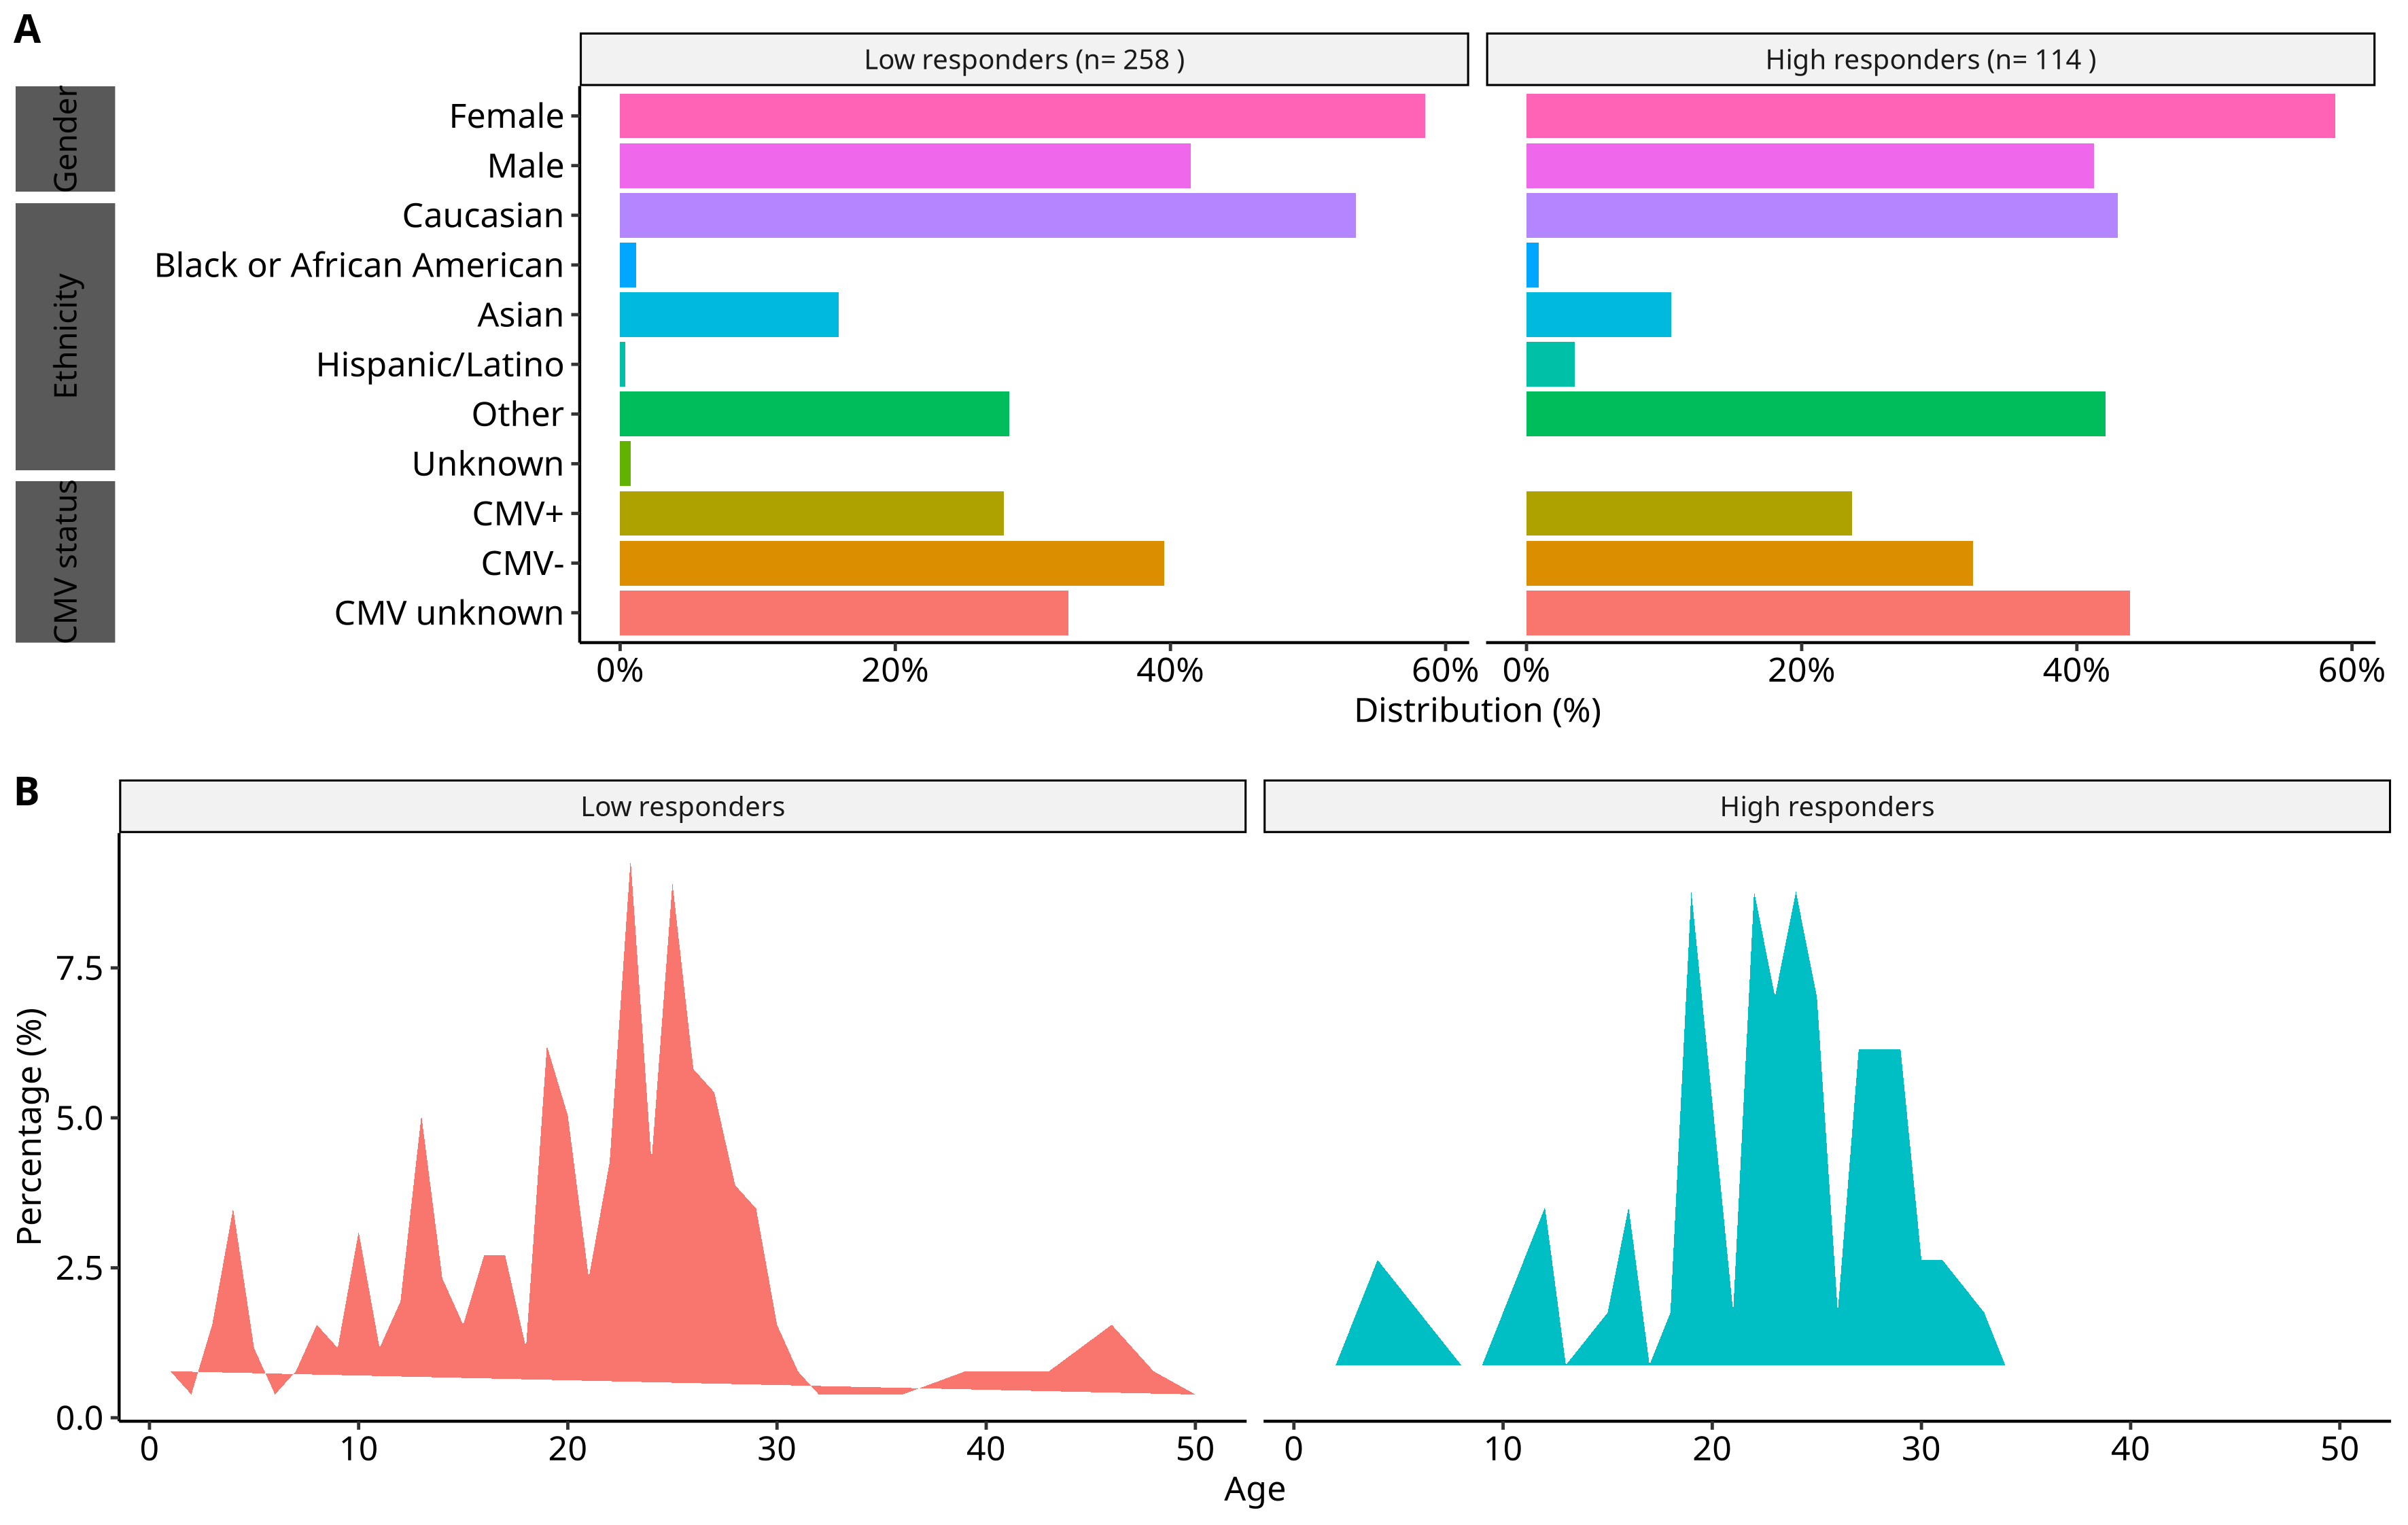
\includegraphics[width=\textwidth]{demographic}
    \label{fig:demoResponder}
    \caption{\textbf{A.} percentage of donors with factor property within high
    and low responder groups. Included are sex, race, and CMV status
    information. \textbf{B.} Age distribution of donors with a known response
    classification.}
\end{figure}

\begin{table}
\centering
\begin{tabular}{ll}
\toprule
\textbf{Age (y)} & \\
\midrule
Mean $\pm$ SD & 21.02 $\pm$ 8.66\\
Median (min. to max. range) & 22.5  ( 1 - 50 )\\
\addlinespace
    \textbf{Gender} & \\
\midrule
Male (\%) & 154 ( 41.4 )\\
Female & 218  ( 58.6 )\\
\addlinespace
    \textbf{Ethnicity} & \\
\midrule
Caucasian (\%) & 187 ( 50.3 )\\
African American (Black) (\%) & 4  ( 1.1 )\\
Asian (\%) & 53  ( 14.2 )\\
Hispanic/Latino (\%) & 5  ( 1.3 )\\
Other (\%) & 121  ( 32.5 )\\
Unknown (\%) & 2  ( 0.5 )\\
\bottomrule{}
\end{tabular}
    \caption{\textbf{Demographic statistics of donors with known vaccine response classification.}}
\end{table}


\citep{chattopadhyaySinglecellTechnologiesMonitoring2014}
The complex heterogeneity of cells, and their interconnectedness with each
other, are major challenges to identifying clinically relevant measurements
that reflect the state and capability of the immune system. Highly multiplexed,
single-cell technologies may be critical for identifying correlates of disease
or immunological interventions as well as for elucidating the underlying
mechanisms of immunity. Here we review limitations of bulk measurements and
explore advances in single-cell technologies that overcome these problems by
expanding the depth and breadth of functional and phenotypic analysis in space
and time. The geometric increases in complexity of data make formidable hurdles
for exploring, analyzing and presenting results. We summarize recent approaches
to making such computations tractable and discuss challenges for integrating
heterogeneous data obtained using these single-cell technologies.

\citep{galliEndOmicsHigh2019}
High-dimensional single-cell (HDcyto) technologies, such as mass cytometry
(CyTOF) and flow cytometry, are the key techniques that hold a great promise
for deciphering complex biological processes. During the last decade, we
witnessed an exponential increase of novel HDcyto technologies that are able to
deliver an in-depth profiling in different settings, such as various autoimmune
diseases and cancer. The concurrent advance of custom data-mining algorithms
has provided a rich substrate for the development of novel tools in
translational medicine research. HDcyto technologies have been successfully
used to investigate cellular cues driving pathophysiological conditions, and to
identify disease-specific signatures that may serve as diagnostic biomarkers or
therapeutic targets. These technologies now also offer the possibility to
describe a complete cellular environment, providing unanticipated insights into
human biology. In this review, we present an update on the current cutting-edge
HDcyto technologies and their applications, which are going to be fundamental
in providing further insights into human immunology and pathophysiology of
various diseases. Importantly, we further provide an overview of the main
algorithms currently available for data mining, together with the conceptual
workflow for high-dimensional cytometric data handling and analysis. Overall,
this review aims to be a handy overview for immunologists on how to design,
develop and read HDcyto data.

\citep{simoniMassCytometryPowerful2018}
Advancement in methodologies for single cell analysis has historically been a
major driver of progress in immunology. Currently, high dimensional flow
cytometry, mass cytometry and various forms of single cell sequencing-based
analysis methods are being widely adopted to expose the staggering
heterogeneity of immune cells in many contexts. Here, we focus on mass
cytometry, a form of flow cytometry that allows for simultaneous interrogation
of more than 40 different marker molecules, including cytokines and
transcription factors, without the need for spectral compensation. We argue
that mass cytometry occupies an important niche within the landscape of
single-cell analysis platforms that enables the efficient and in-depth study of
diverse immune cell subsets with an ability to zoom-in on myeloid and lymphoid
compartments in various tissues in health and disease. We further discuss the
unique features of mass cytometry that are favorable for combining multiplex
peptide-MHC multimer technology and phenotypic characterization of antigen
specific T cells. By referring to recent studies revealing the complexities of
tumor immune infiltrates, we highlight the particular importance of this
technology for studying cancer in the context of cancer immunotherapy. Finally,
we provide thoughts on current technical limitations and how we imagine these
being overcome.

\printbibliography
\end{document}
